%  A simple AAU report template.
%  2015-05-08 v. 1.2.0
%  Copyright 2010-2015 by Jesper Kjær Nielsen <jkn@es.aau.dk>
%
%  This is free software: you can redistribute it and/or modify
%  it under the terms of the GNU General Public License as published by
%  the Free Software Foundation, either version 3 of the License, or
%  (at your option) any later version.
%
%  This is distributed in the hope that it will be useful,
%  but WITHOUT ANY WARRANTY; without even the implied warranty of
%  MERCHANTABILITY or FITNESS FOR A PARTICULAR PURPOSE.  See the
%  GNU General Public License for more details.
%
%  You can find the GNU General Public License at <http://www.gnu.org/licenses/>.
%
\input{setup/preamble.tex}% package inclusion and set up of the document
\input{setup/hyphenations.tex}% 
\input{setup/macros.tex}% my new macros

\begin{document}
%frontmatter
\pagestyle{empty} %disable headers and footers
\pagenumbering{roman} %use roman page numbering in the frontmatter
%  A simple AAU report template.
%  2015-05-08 v. 1.2.0
%  Copyright 2010-2015 by Jesper Kjær Nielsen <jkn@es.aau.dk>
%
%  This is free software: you can redistribute it and/or modify
%  it under the terms of the GNU General Public License as published by
%  the Free Software Foundation, either version 3 of the License, or
%  (at your option) any later version.
%
%  This is distributed in the hope that it will be useful,
%  but WITHOUT ANY WARRANTY; without even the implied warranty of
%  MERCHANTABILITY or FITNESS FOR A PARTICULAR PURPOSE.  See the
%  GNU General Public License for more details.
%
%  You can find the GNU General Public License at <http://www.gnu.org/licenses/>.
%
\pdfbookmark[0]{Front page}{label:frontpage}%
\begin{titlepage}
  \addtolength{\hoffset}{0.5\evensidemargin-0.5\oddsidemargin} %set equal margins on the frontpage - remove this line if you want default margins
  \noindent%
  \begin{tabular}{@{}p{\textwidth}@{}}
    \toprule[2pt]
    \midrule
    \vspace{0.2cm}
    \begin{center}
    \Huge{\textbf{
      Using Grid Computing for Big Data% insert your title here
    }}
    \end{center}
    \begin{center}
      \Large{
        Sorting in a Grid System% insert your subtitle here
      }
    \end{center}
    \vspace{0.2cm}\\
    \midrule
    \toprule[2pt]
  \end{tabular}
  \vspace{4 cm}
  \begin{center}
    {\large
      Project Report%Insert document type (e.g., Project Report)
    }\\
    \vspace{0.2cm}
    {\Large
      Group 12%Insert your group name or real names here
    }
  \end{center}
  \vfill
  \begin{center}
  Aalborg University\\
  Department of Computer Science
  \end{center}
\end{titlepage}
\clearpage
%\input{sections/0.Frontpage/colophon}
\pdfbookmark[0]{English title page}{label:titlepage_en}
\begin{spacing}{1}

\aautitlepage{%
  \englishprojectinfo{
    Using Grid Computing for Big Data\\ %title
  }{%
    A Larger Program Developed by a Group %theme
  }{%
    Spring Semester 2023 %project period
  }{%
    cs-23-sw-2-12 % project group
  }{%
    %list of group members
    Andreas Buje Møller \\
    Christoffer Gamél \\
    Daniel Bødker \\
    Lasse Fonager Hansen \\
    Martin Phutsorn Nielsen \\
    Viktor Dahl Johnsen \\
    Vincent Kosteyev Bechmann
  }{%
    %list of supervisors
    Ramoni Ojekunle Adeogun
  }{%
    \today
  }
}{%department and address
  \textbf{Department of Computer Science}\\
  Aalborg University\\
  \href{http://www.cs.aau.dk}{http://www.cs.aau.dk}
}{
  This project report addresses the problem of sorting big-data using a grid computing system. A web-based system has been developed as a proof of concept using a combination of web-programming and sorting algorithms analysis. The developed program allows users to upload large data sets containing numeric values to be sorted and uses the divide-and-conquer strategy involving splitting of the data into buckets and distribution to worker nodes via a master node, sorting of the data in each bucket at worker nodes and writing the buckets with sorted data, into a file in the server, at the master node.
}

\end{spacing}
\cleardoublepage
\pdfbookmark[0]{Contents}{label:contents}
\pagestyle{fancy} %enable headers and footers again
\tableofcontents
\chapter*{Preface\markboth{Preface}{Preface}}\label{ch:preface}
\addcontentsline{toc}{chapter}{Preface}

This project is made by group cs-23-sw-2-12, a software group from Aalborg University. The project is made with the theme "A Larger Program Developed by a Group". The goal is to make a large-scale program of high quality, that solves a problem found via a problem analysis.
This project was made with guidance from Ramoni Ojekunle Adeogun to whom the group is thankful for his guidance.

The finished product is hosted on \href{https://cs-23-sw-2-12.p2datsw.cs.aau.dk/node0/}{https://cs-23-sw-2-12.p2datsw.cs.aau.dk/node0/}, and the source code of the project can be found on \href{https://github.com/VinceAAU/P2}{https://github.com/VinceAAU/P2}.



\vspace{\baselineskip}\hfill Aalborg University, \today

\newpage
\null
\vfill%\noindent

\begin{minipage}[b]{0.45\textwidth}
 \centering
  Andreas Buje Møller\\
 {\footnotesize <abmo22@student.aau.dk>}
\end{minipage}
\hfill
\begin{minipage}[b]{0.45\textwidth}
 \centering
  Christoffer Gamél\\
 {\footnotesize <cgamel22@student.aau.dk>}
\end{minipage}

\vspace{2\baselineskip}

\begin{minipage}[b]{0.45\textwidth}
 \centering
  Daniel Bødker\\
 {\footnotesize <dbodke@student.aau.dk>}
\end{minipage}
\hfill
\begin{minipage}[b]{0.45\textwidth}
 \centering
  Lasse Fonager Hansen\\
 {\footnotesize <lha22@student.aau.dk>}
\end{minipage}

\vspace{2\baselineskip}

\begin{minipage}[b]{0.45\textwidth}
 \centering
  Martin Phutsorn Nielsen\\
 {\footnotesize <mpni22@student.aau.dk>}
\end{minipage}
\hfill
\begin{minipage}[b]{0.45\textwidth}
 \centering
  Viktor Dahl Johnsen\\
 {\footnotesize <vjohns22@student.aau.dk>}
\end{minipage}

\vspace{2\baselineskip}

\begin{center}
\begin{minipage}[b]{0.45\textwidth}
 \centering
  Vincent Kosteyev Bechmann\\
 {\footnotesize <vbechm22@student.aau.dk>}
\end{minipage}
\end{center}
\cleardoublepage
%mainmatter
\pagenumbering{arabic} %use arabic page numbering in the mainmatter
\chapter{Introduction}\label{ch:introduction}

In contemporary society information is valuable. The spread of the personal computer has created new avenues for information to emerge within people's lives. Within computer science, the word "data" refers to formalised information that can be processed by a machine. Interests, online shopping carts, social circles, and many more, are all pieces of data that can be used as a means to any number of arbitrary ends. However, using data to advance knowledge of a specific area of interest requires the data to be manipulated, for instance, sorted in specific ways to ensure a useful data representation and application \cite{data_ref}.

Given all the possible applications of data collected from people's devices, the sheer volume of data can create issues for traditional data processing techniques \cite{big_data_oracle}. Herein lies the need for more computational power to handle this processing. When expanding computational resources, it is worth considering how to handle it. It is both possible to do vertical and horizontal scaling. Vertical scaling refers to expanding the capabilities of one's computer or node, whereas horizontal scaling refers to adding new nodes to one's system to distribute the workload \cite{scaling_geeks}.


Vertical scaling, while easy in terms of installation, presents several downsides, such as the cost of acquiring new equipment and possessing a single point of failure. Horizontal scaling has the benefit of being able to expand the available processing powers with devices already in one's possession, for instance by making a grid of computational devices which all share resources. However, using a system of distributed computing, like grid computing, requires the development of resource management systems to function properly \cite{TaskSchedulingReview}.

To attain a deeper understanding of this problem and the challenges it presents, this project will explore grid computing as a form of horizontal scaling intended to achieve increased computational power, specifically, exploring how to satisfactorily answer the question: "How can we develop a grid computing system that can sort big data and verify the correctness of the result?".




\chapter{Problem Analysis}\label{ch:problem_analysis}

The purpose of the following chapter is to explore he overall problem domain of grid computing to gain a greater knowledge and understanding of it, so that a narrow and precise problem statement can eventually be formulated.
    \section{Grid Computing}
Grid computing is a type of computing infrastructure where multiple computers work together to achieve a common goal. Unused resources from multiple computers are utilised together to perform a task that is usually extremely large or to solve complex problems, which would otherwise be too demanding for a single computer. Resources such as processing power, storage, and memory are shared across multiple machines. Grid computing has several applications, some of which are analysing designs, performing simulations, financial services, and weather modelling.\cite{AWS_grid_computing}

Computers or servers on a grid are called nodes. There is no limit to the number of nodes a grid can have. There are three types of nodes. These nodes are referred to as master nodes, worker nodes, and user nodes, in this report. There is also middleware, which is a computer program that connects different computers in a grid system together. It helps manage how much processing power each node uses and ensures that no single node utilises too much as this could cause problems for other nodes. The grid middleware can also provide security and prevent nodes from misusing the resources. Often the middleware would be located on the master node, where it is used to assign tasks to the other nodes in the system. 

A worker node is a node that provides computational power to help in the grid. The user node is the one requesting help with a task, that is provided to the grid, as shown in figure \ref{fig:Grid computing illustration} as either a desktop or laptop PC. The user node sends a task it wants fulfilled to the master node which is in the centre \cite{AWS_grid_computing}. Subsequently, as depicted in the illustration, the master node distributes the task to the nodes located in the upper, right, and lower locations, highlighting that the task is distributed throughout the system. 

\begin{figure}[H]
    \centering
    \includegraphics[scale=0.60]{figures/Grid-Computing.jpg}
    \caption{ 
    A visualisation of what a grid computing system could look like. In this illustration, the Master node is called Control node \cite{Gridcomputing_image}.}
    \label{fig:Grid computing illustration}
\end{figure}

When creating a grid computing system, there are several factors that need to be fulfilled to have an optimal system. When assessing how optimal the system is, it is important to keep the limits that the system needs to work within in mind. For example, if running time is important, one would need to set a limit for the time the system is allowed to run for. This is referred to as temporal verification.
Other things that are relevant to optimise are structure verification, performance verification, and resource verification.

Structure verification refers to the verification of the system's structure and the way the system is set up. This includes both the semantic and syntactic structure of a given system. The syntactic part of the system includes problems such as lack of synchronisation, general misuse of the structure, deadlock, where some nodes are effectively blocking each other since they are trying to reach each other's resources, and livelock, where the nodes are constantly changing their own output, since the other node that it needs work from changes.
The semantic part is also important. Suppose a system works in terms of syntax and a task needs to be done in either node A or B, but the semantics of the system decide that node C, even though it is nonexistent, would be a better option. For the structural integrity of the system, it is important to avoid such a scenario \cite{grid_workflow_validation}.

Another thing that needs to be verified in the system is its performance. This is called the verification process, where the system is tested within user-defined parameters, such as an average completion time, average capacity, synchronisation delay, average resource allocation, and so on. This can be tested either on each node in the system or on the whole system in general. There are multiple ways, this can be achieved, such as the Markovian chain theory, the queuing theory, or simulation tools, with each their advantages and disadvantages \cite{grid_workflow_validation}.

Another type of verification that is important to have in the system, is resource verification. This is a process where the system is tested to ensure that it distributes the data that it gets efficiently and the resources of the system are handled correctly. Ensuring that nodes are not trying to compute the same data and that the resources are not distributed to the same node \cite{grid_workflow_validation}.
    \section{Big Data}
Big data often refers to exceedingly large and complex data, often characterized by three V's: volume, velocity, and variety. Depending on the organisation, when talking about big data, the volume can be anywhere from terabytes to petabytes. Companies working with big data usually also get the data at a high velocity, and depending on the company that uses the data, the company might also need it to move at a high velocity. Data can come from several different types of sources. Due to this, it may need to be processed in near real-time to be used effectively. When gathering data, the data can come in a variety of formats and a lot of these data types are unstructured or semi-unstructured \cite{big_data_oracle}.

\subsection{Problems with big data}
Some of the problems with big data is its massive volume which makes it hard to store. Furthermore, data has to be processed, from raw information to useful information, in order to be efficiently used. This can be a problem as it takes a lot of work. A data scientist can spend between 50 to 80 percent of their time on just preparing data \cite{big_data_oracle}. This takes a lot of processing power that can be costly to have. Another problem when it comes to big data is security, which is a significant concern for organisations. When information is left unencrypted it is at a high risk of being stolen or compromised by a malicious actor. This can become an issue if not handled correctly, as one still needs to access the data without putting it at risk.

\subsection{Why is grid computing relevant for big data}
Grid computing can be a good solution for the problems big data has, as it enables the processing of massive volumes of data in a distributed manner. Considering the massive volume, velocity, and variety of data, processing it all could be too much for a single machine. While giving a lot of processing power, grid computing could also result in faster processing times and more efficient use of resources. This becomes especially relevant in organisations where information needs real-time analysis to keep up.
    \section{Challenges in Grid Computing}

When handling big data in a distributed system, such as a grid computational system, some important challenges have to be taken into account to ensure the reliability of the application. This includes challenges such as task scheduling, node failure, malicious intent, validation, authentication, and authorization.
    \subsection{Task Scheduling}
In a grid computing system, tasks must be scheduled to the worker nodes appropriately so as to not waste the resources offered by the grid. Grids use a task scheduler to achieve this. The task scheduler is responsible for receiving, keeping track of, and delegating jobs to the worker nodes, ideally, finding the most suitable node for the job in question. There are several ways to structure a task scheduler, each with its own advantages and disadvantages \cite{TaskSchedulingReview}.

\subsubsection{Centralized Scheduling}
In a centralized system, the tasks are distributed to the worker nodes by a server. This is a relatively simple way of creating a task scheduler, but it has some weaknesses. For large systems with many job requests and nodes, the master node itself can require significant computational resources for the task of scheduling, which can cause a bottleneck and ultimately lead to inefficiency. A centralized system is also prone to system failure, as the entire system will cease working if the server fails. This type of system scales vertically, as the central unit will have to be upgraded to handle more nodes. Centralized systems are mostly used for their cost-effectiveness in relatively small grids and their ease of use. Having a centralized unit also makes security issues simpler to solve. \cite{TaskSchedulingReview, SchedulingInGridComputing}.

\subsubsection{Distributed Scheduling}
In distributed scheduling, there is no central unit issuing orders to the worker nodes in the system. This can be done by allowing each node to communicate with all other nodes in the grid for information about their availability and workload and using a local scheduler to determine the appropriate task to start. This type of scheduling prevents system-wide failure from a single node failing. If a node fails, another node will eventually complete the job. This, however, does not prevent a distributed scheduling system from producing a faulty result, as it can be difficult to implement proper validation of completed jobs. This system also requires more communication between nodes than centralized scheduling, which can cause a bottleneck as the number of nodes increases \cite{SchedulingInGridComputing, Systems_geeks}.

\subsubsection{Hierarchical Scheduling}
As opposed to distributed and centralized scheduling, hierarchical scheduling uses more than two types of nodes. This system works by dividing the grid into several sub-grids using a main scheduler node and handing over command to several manager nodes. The hierarchy can then be expanded with more intermediate manager nodes for more localization. Depending on implementation, this type of scheduler can still be prone to system-wide failure, if the main scheduler node fails. However, the system will not fail completely, as the rest of the grid can handle any jobs in queue, but they may not be able to accept new jobs. As the main scheduler has a minimal workload, and all other nodes' workload can be lessened by simply adding more nodes, this scheduler scales well horizontally \cite{Behnam1330, TaskSchedulingReview}.

\subsubsection{Resource-based Scheduling}
Nodes will often have vastly different capabilities in terms of processing power, especially in volunteer grid computing systems. This can lead to inefficiency if not taken into account during task scheduling. If each node is assigned a similar task, the slower nodes will slow down the whole system, while the fast nodes idle. There are several ways to account for this depending on the type of scheduler used. The biggest issue with optimizing for worker resources is the communication overhead. Taking the capabilities of each node into account often requires frequent communication between the scheduler and worker nodes, as the processing power is subject to change. If the owner of a worker node in a volunteer grid computing system opens another resource intensive task, it may fall behind on its task assigned by the scheduler, leading to it slowing down the system. To avoid this, communication between the worker nodes and the scheduler(s) must be maintained actively, and not just at the start of a task \cite{abhang_2012}.
    \subsection{Node Failure} \label{sec:nodeFailure}

When there are a large amount of nodes in a system, and they are used to process a large amount of data, it is inevitable that some of them will fail, and therefore it is imperative that a grid computing system is able to deal with these issues.

\subsubsection{Detection}

The first step to dealing with node failure is to detect that the node has failed.

One way to detect node failure is by monitoring the network itself.
However, this requires detailed knowledge about the network that the nodes operate on, which is not reasonable to have if you have a large number of nodes spread over a large variety of networks with different properties \cite{dabrowski_2009}.

Another way is through heartbeat techniques, where nodes will occasionally ping each other to make sure that no worker node has disconnected. This technique is common, as it can be implemented quite simply, and will work even in diverse and dynamic environments. In a distributed system, this has the drawback that it does not scale well, as each node must always communicate with every other node. Trying to centralise the heartbeat creates a single node that acts as a hot-spot, and heartbeating in a ring creates unpredictable fail detection times
\cite{gupta_chandra_goldszmidt_2001}.

\subsubsection{Mitigation}

When a node fails, it might either be a temporary failure (e.g. due to network failures, or unexpected software updates) or a permanent failure. 

If a node is temporarily down and therefore ends up missing some of the tasks, it must communicate with its master about where it last left off, so that it can catch up to all those tasks, and continue from there. This requires that the worker keeps a note of which message it has last received and that the master node keeps a journal of its previously distributed tasks. 

However, if a node is permanently down, its tasks must be redistributed entirely. This once again requires that the master node keeps a journal of previously distributed tasks, so it can redistribute the ones given to the failed node, to a node that is still in operation. 

If the failed node is a master node, a new master could be elected. In the case of a faulty election or bad communication, two masters might be elected, which would result in a split brain. This should be avoided. After an election, the new master must be able to continue from where the previous one has left off. This might be a challenge if the worker node does not have a properly updated list of tasks, which is likely due to the asynchronous nature of grid computing \cite{upadhyay_2021}.

    \subsection{Malicious Intent}
Another thing that is not necessarily inevitable, but a thing that one should worry about, is the presence of malicious intent in one's grid computing system. It is important that the system can detect and handle such intent.

In the context of this report, malicious intent is when some outside force or a node within the system, tries to disrupt the flow of the working grid. Some examples of malicious intent could be when attackers try to take the resources utilized by the grid and use them for their own gain, or when the attackers try to make a worker node create a false or invalid result, or in some way spread viruses among the nodes in the grid \cite{detecting_malicious_manipulation}.

There exist many different ways of detecting and catching malicious nodes, one method is a system-level diagnosis, where the system sends ping-messages to the nodes containing tests and through these tests, the system can detect malicious or faulty nodes. A classic example of such a diagnosis is the Preparata-Metze-Chien (PMC) diagnosis, where a test is sent out to multiple nodes and the result is then checked at the master node. If all the nodes give the same result, they are considered non-malicious, but if one gives a different result from others it is considered malicious and should be dealt with \cite{detecting_malicious_manipulation}.

Malicious intent can be seen as a form of security hacking and the motives for creating malicious nodes and hacking are very similar. One motive could be monetary gain. Attackers could achieve this in a number of ways, such as using the data that they gather to blackmail or extort money from either a corporation or a person. Another way that attackers could obtain money could be through selling the data that was obtained illegally. If they get data from a company they could sell the data to other competing companies or if they get data from a private person they could sell it to companies who would want such data \cite{why_do_hackers_hack}.
    \subsection{Authentication \& Authorisation}
Sending data from one node to another in a grid computing system can cause problems. These transfers can be the target of malicious attacks or nodes can present themselves as a trusted node, without being a trusted node itself. This makes it important to authenticate the different nodes, so that the identity of each node is checked and validated. 

\subsubsection{Certificate Authority (CA)}
One way to ensure that both nodes involved in a data transfer are authenticated is by using a certificate authority (CA). This is a trusted node that is responsible for checking and entrusting new nodes. This is done with a two-key encryption system with a public and a private key. Every node has its own set of keys. The private key is kept safe by that node, and no one else should know that key, while the public key is known by anyone who wants it. This is also the case for the CA node. When adding a new node to the network, that node would then provide a certificate with the information about the node, containing the public key of the node, to the CA node. The CA node would then check the information and if everything is in order, it would then sign it with its private key. This means that from now on the new node would be able to show this certificate and other nodes could verify that this node has been checked by the CA node since they can use the CA public key to decrypt the encrypted signature of the CA node. The node that checked the signature can then use the public key on the certificate to encrypt and transfer data to the node that had the certificate. This certification can be shared and copied without any risk, as only the node that originally got the certificate can use it. This is because anything encrypted by the public key on the certificate can only be decrypted by the private key that only that one node knows \cite{IBM}.

This means that any transfer between two nodes would be as follows. Node A sends a certificate to node B. Node B checks the certificate. Node B then sends its certificate, which is verified by node A. Both nodes have now been verified. Node A will then encrypt its data, first with its own private key, then with the recipient's public key. This method ensures that only the intended recipient, in this case, node B, can access the data, as only they possess the private key that matches the public key on their certificate. It also ensures that node A is the sender, as only their public key will decrypt what was encrypted with their private key. It is therefore very hard to access the data for anyone who might have intercepted the transfer \cite{IBM}.

When dealing with larger systems, some of the tasks that the CA node handles might be handed off to another node. This node is known as a registrant authority (RA). The RA node takes care of checking whether the information on a not yet signed certificate is correct, before it is handed over to the CA node to lessen the workload of the CA node \cite{IBM}.

\subsubsection{Attribute Based Authorisation}
Different nodes in a grid may have different tasks or may be trusted on different levels. You may need to have nodes that are only workers, nodes that can provide work tasks, and nodes that can distribute tasks. This is done by granting different nodes authority to complete certain tasks. The simplest version of this is keeping track of exactly what every single node is allowed to do, so they can be granted access to these tasks after they have been authenticated. This works well for small grids but is not very scalable, as grids can have hundreds of nodes, and you then have to keep track of permissions individually. Another solution for this is to use an attribute-based authorisation system. This system is built on creating and assigning different roles. This might be a worker, a task scheduler, and a work provider. Nodes in the same group would have the same authorisation level and can therefore just be assigned as a worker. The system would then know what a worker is allowed to do without having to check or store the specific nodes' authorisation. This also has the benefit of being able to edit authorisation in one central place instead of having to change it for every single node \cite{4144613}.

    \section{Problem Delimitation}
During the problem analysis, multiple areas of big data and grid computing have been explored. This was done to specify a focus area of the initial problem statement. A concept map was created to get an overview of the different problems that exist when working with big data and problems related to grid computing. This is what is shown in figure \ref{fig:concept_map}. As seen in the initial problem statement, the focus was initially on developing a grid computing system where an implementation of a sorting algorithm would be created, that would also verify the correctness of the given result. During the process analysis, the scope and relevance of these areas were discovered. Because of this, one area was chosen to focus on. The only part that will be focused on in this project is the sorting part of the grid computing system and validation will not be a focus.


\begin{figure}[H]
    \centering
    \includegraphics[scale=0.95]{figures/concept_map.png}
    \caption{Concept map of problems regarding big data.}
    \label{fig:concept_map}
\end{figure}
    \section{Problem Statement} \label{sec:problemStatement}
During the problem analysis, it became obvious that the scope of the project should be limited to only one of the problems included in the initial problem statement. This means that the project will focus on time-efficient sorting of data for a grid computing system leading to the following problem statement:

\begin{center}
\emph{How can a web-based software solution be developed for time-efficient sorting of big data on a grid computing system?}
\end{center}

Validating the correctness of the result, security, authentication, and authorization will instead be secondary priorities that will enhance the quality of the product without being essential for the success of the project.
\chapter{Software Design}\label{ch:SoftwareDesign}

This chapter presents the software requirements as well as modelling and design to satisfy the final problem statement in Section \ref{sec:problemStatement}. The different parts of the software, as well as the interactions between them, are described



    \section{System Overview}
In order to develop a piece of software that achieves the specifications of the problem statement, this chapter will include all the system requirements made for the product. 

Block diagrams will be used to show an outline of the different parts of the system. The MoSCoW method will be used to manage the requirements that exist for the product. 

This is done so as to have a clear understanding of what is important for the product, and which requirements are more highly prioritised than others, while still touching on other possible features for the product. 

\begin{figure}[H]
    \adjustbox{scale=0.75, center}{
        \begin{tikzpicture}[node distance=5cm,
            component/.style={draw, text width=2cm, text centered, node distance=2cm},
            important_component/.style={draw, text width=4cm, text centered}]
            
            \node [important_component] (frontend) {Frontend};
            \node [important_component] (backend) [right of=frontend, xshift=3cm] {Backend};

            \node [component] (customer) [below of=frontend, xshift=-2cm] {Customer};
            \node [component] (worker) [below of=frontend, xshift= 2cm] {Worker};

            \node [component] (server) [below of=backend, xshift=-2cm] {Server};
            \node [component] (master) [below of=backend, xshift= 2cm] {Master};

            \node [component] (filesystem) [below of=master, xshift=-2cm] {Filesystem};
            \node [component] (tasks) [below of=master, xshift= 2cm] {Tasks};

            \node [component] (fetch) [below of=server, xshift=-2cm] {Router};  


            \draw[<->] ([xshift=3pt]frontend.east) -- ([xshift=-3pt]backend.west);

            \draw[->] ([yshift=-0.5pt, xshift=-1cm] frontend.south) -- ([yshift=3pt]customer.north);
            \draw[->] ([yshift=-0.5pt, xshift=1cm]frontend.south) -- ([yshift=3pt]worker.north);

            \draw[->] ([yshift=-0.5pt, xshift=-1cm]backend.south) -- ([yshift=3pt]server.north);
            \draw[->] ([yshift=-0.5pt, xshift=1cm]backend.south) -- ([yshift=3pt]master.north);

            \draw[->] ([yshift=-0.5pt, xshift=-1cm]master.south) -- ([yshift=3pt]filesystem.north);
            \draw[->] ([yshift=-0.5pt, xshift=1cm]master.south) -- ([yshift=3pt]tasks.north);         

            \draw[->] ([yshift=-0.5pt, xshift=-1cm]server.south) -- ([yshift=3pt]fetch.north);              
            
            \draw[frame=33pt];
        \end{tikzpicture}
    }

    \caption{A block diagram providing an overview of the system.}
    \label{fig:SystemOverview}
\end{figure}
Figure \ref{fig:SystemOverview} outlines the main points of the system. 

Under the backend are the server and master. The server is responsible for serving the web-pages to the frontend interface. The master is the system that divides data into tasks, and distributes it among workers.

Under the frontend, are the customer and worker pages. The customer in question is the user that needs their files sorted, and the customer page is therefore the interface through which said user can upload the files that need sorting. The worker receives tasks from the master, and completes said tasks, before sending the processed data back. 

\subsection{Frontend Overview}

\begin{figure}[H]
    \adjustbox{scale=0.75, center}{
        \begin{tikzpicture}[node distance=4cm,
            webpage/.style={draw, text width=4cm, text centered}]

            \node[webpage] (index)                                                         {Index};

            \node[webpage] (login)               [below of=index]                          {Login};

            \node[webpage] (createUserRight)     [right of=login, yshift= 1cm, xshift=2cm] {Create User};

            \node[webpage] (forgotPasswordRight) [right of=login, yshift=-1cm, xshift=2cm] {Forgot Password};

            \node[webpage] (worker)              [below of=login, xshift=-3cm]             {Worker};

            \node[webpage] (customer)            [below of=login, xshift= 3cm]             {Customer};
    
            \draw[->] ([xshift=-1cm]index.south) -- ([xshift=-1cm, yshift=3pt]login.north);
            \draw[->] ([xshift= 1cm]index.south) -- ([xshift=1cm, yshift=3pt]login.north);

            \draw[->] ([xshift=-1cm]login.south) -- ([yshift=3pt]worker.north);
            \draw[->] ([xshift= 1cm]login.south) -- ([yshift=3pt]customer.north);

            \draw[<->] ([xshift=5pt]worker.east) -- ([xshift=-5pt]customer.west);

            \draw[<->] ([xshift=3pt, yshift=5pt]login.east) -- ([xshift=-3pt]createUserRight.west);
            \draw[<->] ([xshift=3pt, yshift=-5pt]login.east) -- ([xshift=-3pt]forgotPasswordRight.west);


            \draw[frame=33pt];
        \end{tikzpicture}
    }

    \caption{A block diagram providing an overview of the frontend aspect of the website.}
    \label{fig:frontendOverview}
\end{figure}

In order to make an overview of the parts within the product's user interface, a block diagram was made (Figure \ref{fig:frontendOverview}). This is not a detailed diagram, but it gives an overview of what is encompassed in the user interface of the product's frontend. As can be seen in the figure, there are two arrows from the "Index" block to the "Login" block. This is due to the fact that a dynamic login system will be implemented, such that when the user wants to navigate to either the customer or worker page, they will first be directed to the login page and afterwards redirected to the desired page.

\subsection{Backend Overview}
\begin{figure}[H]
    \adjustbox{scale=0.75, center}{
        \begin{tikzpicture}[node distance=5cm,
            component/.style={draw, text width=2cm, text centered, node distance=2cm},
            important_component/.style={draw, text width=4cm, text centered}]
            
            \node [important_component] (upload) {Upload File};

            \node [component] (save) [below of=frontend, xshift=-2cm] {Save to Server};
            \node [component] (queue) [below of=frontend, xshift=2cm] {Queuing System};

            \node [component] (task) [right of=queue, xshift=2cm] {Task Splitter};
            \node [component] (scheduler) [right of=task, xshift=2cm] {Task Scheduler};

            \node [component] (worker) [above of=scheduler] {Worker};

            \draw[->] ([yshift=-0.5pt, xshift=-1cm] upload.south) -- ([yshift=3pt] save.north);
            \draw[->] ([yshift=-0.5pt, xshift=1cm] upload.south) -- ([yshift=3pt] queue.north);

            \draw[->] ([xshift=0.5pt] queue.east) -- ([xshift=-3pt] task.west);
            \draw[->] ([xshift=0.5pt] task.east) -- ([xshift=-3pt] scheduler.west);

            
            \draw[->] ([xshift=-0.75cm] worker.south) -- ([yshift=3pt, xshift=-0.75cm] scheduler.north);            
            \draw[->] ([xshift=0.75cm] scheduler.north) -- ([yshift=-3pt, xshift=0.75cm] worker.south);    
            
            \draw[frame=33pt];
        \end{tikzpicture}
    }

    \caption{A more detailed look into the "Tasks" part of the backend model mentioned in Figure \ref{fig:SystemOverview}.}
    \label{fig:BackendOverview}
\end{figure}

The diagram in figure \ref{fig:BackendOverview} gives an overview of how the task-handling part of the backend is structured. The diagram provides an overview of how different parts of the server side interact with each other. The process starts when a customer uploads a file. Once this file is saved to the server, it is put into the file queuing system, where it will stay until the server is ready to work on that file. The file will be split into various tasks which the task scheduler delegates to different workers. This continues until all of the tasks are done. The sorted file is then sent to the list of finished files.

\section{System Requirements} \label{sec:MoSCoW}
This section uses the MoSCoW method to prioritise different, possible features for the development of the product. 

\subsection{MoSCoW Method} 

\subsubsection{Must Have} 
\begin{enumerate}
    \item The master node must be able to receive a task from a customer.
    \item The product must have a web-based user interface, where the customer can upload a CSV document, containing only numbers that need to be sorted.
    \item The master node must be able to split tasks into suitable sizes, such that any modern, consumer-grade device can be a worker node in the system.
    \item The master node must be able to connect, and distribute tasks, to worker nodes.
    \item The grid must be able to handle a minimum of three nodes: one master and two connected worker nodes
    \item The master node must be able to receive results from worker nodes.
    \item The master node must be able to combine results that it receives from the worker nodes.
    \item The master node must be able to return the final product (a sorted CSV document) to the customer.
\end{enumerate}

\subsubsection{Should Have}
\begin{enumerate}
    \item The grid should be able to sort a file efficiently in regards to time.
    \item The master node should be able to validate the results that it receives from the worker nodes.
    \item The product should have a web-based login system so that the identity of a user can be verified, to keep track of their files.
    \item The master node should keep track of tasks, both tasks that are completed and pending.
    \item The master node should validate the type and content of the input CSV file.
\end{enumerate}

\subsubsection{Could Have}
\begin{enumerate}
    \item Login sessions could expire after some time, in order to enhance security.
    \item The login system could have a mechanism for preventing SQL injections and similar attacks.
    \item There could be a reward system for contributing worker nodes.
\end{enumerate}

\subsubsection{Will Not Have}
\begin{enumerate}
    \item The master node will not be able to process two files simultaneously.
    \item The frontend will not have an option for the customer to upload custom scripts for workers to run.
\end{enumerate}

    \section{Frontend Model} 
The program's interface will be a website consisting of several web pages, including an index and login page, a worker page, and a customer page.

\subsection{Index and Login Page}
The login page should contain a simple form asking for a username and password. This page could also contain buttons to create a new user, and a button to change password.
\begin{figure}[H]
    \adjustbox{scale=0.6, center}{
        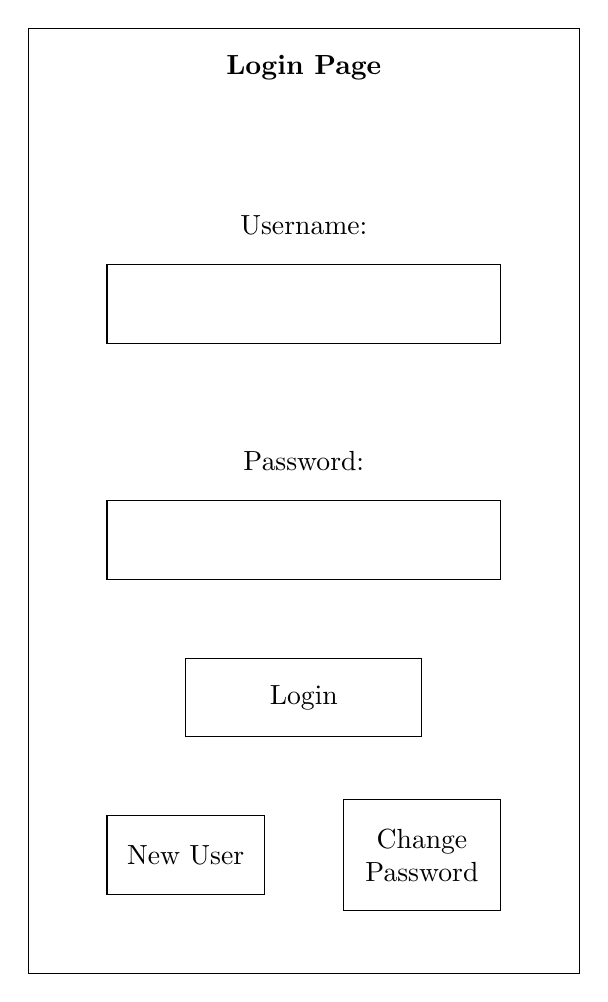
\begin{tikzpicture}
            \draw (0,0) rectangle (7,12);
        
            \draw[font=\bfseries] (3.5, 11.5) node {Login Page};
        
            \draw (3.5, 9.5) node {Username:};
            \draw (1,9) rectangle (6,8);
        
            \draw (3.5, 6.5) node {Password:};
            \draw (1,6) rectangle (6,5);
        
            \draw (2, 4) rectangle (5, 3);
            \draw (3.5, 3.5) node {Login};
        
            \draw (1,1) rectangle (3,2);
            \draw (2,1.5) node {New User};
            \draw (4,0.8) rectangle (6,2.2);
            \draw [align=center] (5, 1.5) node {Change\\Password};
        \end{tikzpicture}
    }
    \caption{An illustration of the login system.}
    \label{fig:LoginPage}
\end{figure}


\subsection{Worker Page}
The worker page should contain a button to toggle whether the worker node is doing work, as shown in Figure \ref{fig:WorkerPage}.

\begin{figure}[H]
    \adjustbox{scale=0.75, center}{
        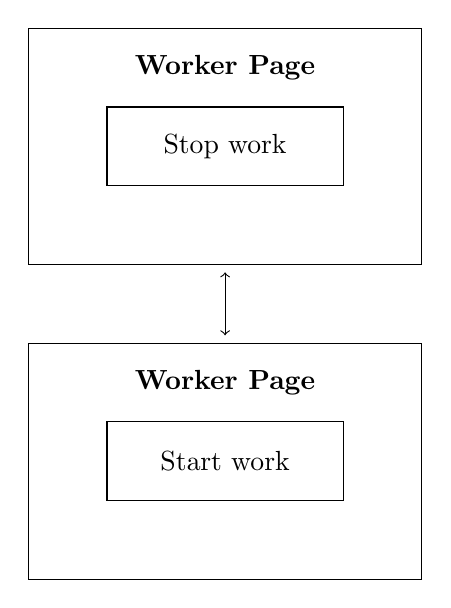
\begin{tikzpicture}
            \draw[font=\bfseries] (2.5,2.5) node {Worker Page};
            \draw(0,0) rectangle (5,3);
            \draw(1,1) rectangle (4,2);
            \draw (2.5, 1.5) node {Start work};
        
            \draw[<->] (2.5,3.1) -- (2.5,3.9);
        
            \draw[font=\bfseries] (2.5,6.5) node {Worker Page};
            \draw(0,4) rectangle (5,7);
            \draw(1,5) rectangle (4,6);
            \draw (2.5, 5.5) node {Stop work}; 
        \end{tikzpicture}
    }
    \caption{An illustration of the worker page.}
    \label{fig:WorkerPage}
\end{figure}


\subsection{Customer Page}
The customer page should interface with the master node. As shown in Figure \ref{fig:CustomerPage}, there should be a button for uploading files for processing, and a list of files ready to be downloaded.

\begin{figure}[H]
    \adjustbox{scale=0.75, center}{
        \usetikzlibrary{patterns}
        \begin{tikzpicture}
            \draw (0,0) rectangle (5,8);
        
            \draw (1,1.2) rectangle (4,1.8);
            \draw (2.5,1.5) node {thirdFile.csv};
        
            \draw (1,2.2) rectangle (4,2.8);
            \draw (2.5,2.5) node {secondFile.csv};
        
            \draw (1,3.2) rectangle (4,3.8);
            \draw (2.5,3.5) node {firstFile.csv};
        
            \draw (2.5, 4.5) node {Ready files download:};
        
            \draw(0.5, 5.5) rectangle (4.5, 5.8);
            \draw[pattern=north east lines](0.5, 5.5) rectangle (2, 5.8);
        
            \draw (1, 6) rectangle (4, 7);
            \draw (2.5,6.5) node {Upload file};
        \end{tikzpicture}
    }
    \caption{An illustration of the customer page.}
    \label{fig:CustomerPage}
\end{figure}
    \section{Sorting on a Grid Computing System}
To effectively sort large amounts of data on a distributed system, the following considerations must be made: 
\begin{itemize}
\item How to divide the data into tasks that can be sent to the worker nodes
\item Which algorithms the workers should use to sort those tasks
\item How to merge the sorted packages into one list
\end{itemize}

The above considerations naturally lead to a divide-and-conquer design process. Bucket Sort was used to divide the data and then merge it back together, and Quicksort was chosen as the worker-side sorting algorithm.

\subsection{Distribution of Data to Worker Nodes} \label{sub:modelSplitData}
The master must split the data into tasks for the workers to process. Ideally, these tasks should be of roughly equal size (as discussed in Section \ref{sec:benchmarking}), not so large that they overwhelm the workers, and not so small that the communication overhead becomes larger than the data processing time.

Traditional divide-and-conquer algorithms like Merge Sort and Quicksort divide the data into as many parts as there are elements, and then gradually combine them until there are two parts left to merge. Simply sending these parts to workers will have communication overhead in the beginning, as packets are very few bytes in size, and gradually the problem will shift to workers being overloaded as packets become almost as large as the original data. 

A much better alternative is to divide the data into a series of intervals called "buckets", as shown in Figure \ref{fig:bucketsort}. In the figure, the buckets range between 0 and 49, and there are five buckets. The first bucket should contain all the numbers between 0 and 9, the second bucket should contain all the numbers between 10 and 19, and so on. The correct bucket can be calculated as $\lfloor\frac{\text{Element}}{\text{Bucket interval}}\rfloor$. This process can be done while the file is being loaded, and has a complexity of O($n$) \cite{Introduction_to_algorithms}. This process has the disadvantage of only being effective on uniform distributions. For example, a Gaussian distribution will lead to large buckets in the middle of the data range, and small buckets near the edges, which is contrary to the goal of uniform-sized data packages. A possible mitigation could be dynamically-ranged buckets, where a bucket that would otherwise contain too much data could be split up into more reasonably-sized buckets, but this is not implemented in this project.

\begin{figure}[h]
    \centering
    \includegraphics[scale=0.25]{figures/Bucketsort.png}
    \caption{An example of bucket sort working on a list and sorting it into 5 buckets.}
    \label{fig:bucketsort}
\end{figure}


\subsection{Sorting of Local Data by Worker Nodes} \label{sec:quicksortDesc}
Frequently, Quicksort is compared to other sorting algorithms, like Mergesort and Heapsort. This is because they share many similarities and excel in similar tasks. The three algorithms all have an average time complexity of O($n\,log\,n$), making them well-suited for efficiently sorting large data sets \cite{Algorithm_sorts_stanford}. Although all three have an average time complexity of O($n\,log\,n$), their worst case time complexities vary. Quicksort has a worst-case time complexity of O($n^2$) while Mergesort and Heapsort both have one of O($n\,log\,n$). Despite this, Quicksort is still typically considered the fastest, when taking hardware considerations into account \cite{Quicksort_better_answer}.


Another important distinction between the sorting algorithms is their space complexity. Heapsort and Quicksort are both algorithms that can perform sorting in-place, meaning they directly manipulate the data they are working with and hence, do not require any extra memory \cite{In-place_guide}.

\subsubsection{How Quicksort works} \label{HowDoesQuicksortWork}
Quicksort is an algorithm that uses the divide-and-conquer strategy. The algorithm works by choosing a pivot point and then running through all the numbers and dividing them into sub arrays of elements smaller than or bigger than the pivot point. Once this step is completed, the pivot point should be sorted correctly in relation to the smaller or larger numbers. This process is then being repeated until every element is sorted. The performance of the algorithm is significantly influenced by the way the pivot point is chosen. Several commonly preferred options include choosing the first or last element, selecting a random element, or using the median of the first, middle, and last element as the pivot point.


The pseudo-code in algorithm \ref{quicksort_algorithm} shows how the Quicksort algorithm can be implemented:

\begin{algorithm} [H] 
\caption{quicksort(left = $0$, right = Data.length $- 1$)} \label{quicksort_algorithm}
\SetAlgoNoLine

\uIf{left $<$ right}{
pivotIndex = genRandomInt(left, right) 

pivot = data[pivotindex] 

partitionIndex = HOARE-PARTITION(pivot,left,right)

quicksort(left, partitionIndex)

quicksort(partitionIndex $+ 1$, right)

}
\Else{
\textbf{return}
}

\end{algorithm}

At the beginning of the sorting process the variables "left" and "right" are initialized with placeholders, where "left" is set to 0 and "right" is set to the length of the data minus one. If "left" is smaller than "right", a pivot point is randomly selected between "left" and "right". Afterwards, the variable "pivot" is set to the value of "data[pivot]" 

Next, the code HOARE-PARTITION (as described in Algorithm \ref{Partition}) runs and returns the index of the partition point to the variable "partitionIndex". This then splits the data in two subarrays, one with every number under the pivot index, and another with every number over the pivot index. The Quicksort algorithm then calls itself twice, once for each of the subarrays created.
\\
Pseudo-code \ref{Partition} shows how Hoare's partition can be implemented \cite{Introduction_to_algorithms}:

\begin{algorithm} [H] \caption{HOARE-PARTITION(pivot, left, right)}\label{Partition}
\DontPrintSemicolon
\SetAlgoNoLine
    x $=$ pivot\\
    i $=$ left $- 1$\\
    j $=$ right $+ 1$\\
     \While{TRUE}{
     \RepeatUntil{A[j] $\le$ x}{j$=$j$-1$}
     \RepeatUntil{A[i] $\ge$ x}{i$=$i$+1$} 
     \If{i $<$ j}{
       Exchange A[i] with A[j]
    }
     \Else{
        \textbf{return J}
    }
}

\end{algorithm}

The pseudo-code demonstrates a single call of the partition function on an unsorted list, using the two pointer approach, also known as Hoare's partition scheme. The way it works is by having two pointers, one at the end and one at the beginning of the array. The pointer at the end goes through all the elements on the right side of the pivot point until it finds a number that is smaller than the pivot. The pointer at the beginning of the array does the same thing afterwards, from the left side of the pivot point, until it finds a number bigger than the pivot. When both conditions are met, the algorithms swaps the two numbers and then continues to check every number until they meet each other. When the algorithm terminates it returns the partition index \cite{hoare-partition}.

\subsection{Merge of Sorted Data at the Master Node}
Once all the workers have finished their tasks and sent the finished buckets back, the buckets must be merged. Because they were split into buckets, where the elements of bucket $n$ are always greater than those of bucket $n-1$, the merge procedure is as simple as concatenating the buckets. 
    \section{Considerations for Task Distribution} \label{sec:benchmarking}

Benchmarking worker nodes to find their computational power can be beneficial for reducing the communication overhead of the grid. However, this is not always the case. Knowing the capabilities of each node allows the task scheduler to assign a node an appropriately sized task. However, finding out what a worker is capable of, without spending more time than would be gained, proves a difficult challenge \cite{Charpentier_2017}.

In the case of this product, the capabilities of the nodes will be somewhat unpredictable, and the processing power of a node may vary greatly while processing an assigned task, due to other processes being opened or closed. For this reason, benchmarking the worker nodes at the start of, or during, a task was considered to optimise the task scheduler. However, the idea of benchmarking nodes continuously was discarded as it simply takes too much time to perform a benchmark, and many benchmarks would need to be done to account for processes being opened and closed \cite{Charpentier_2017}.
Benchmarking a node at the start of a task is more realistic, but it is unclear how useful the information gathered would be. The information would be used to give a node a smaller or larger task relative to other nodes in accordance with its processing power. The benefit of doing so is to reduce the amount of time spent waiting for slower nodes to finish in the grid. However, since the computational power can vary throughout the task, and a node may end up being slower than initially predicted, this can lead to the same problem regardless. \cite{Mengistu2019}

An alternative to benchmarking nodes is to simply send tasks of equal sizes to all worker nodes, regardless of their abilities. If the task is small enough, the time spent waiting for slow nodes will be smaller, which somewhat helps with the issue. However, having smaller packages will result in a larger communication overhead, as nodes will need to request new tasks more often. 
\chapter{Software Implementation}
This chapter will focus on documenting the development process of the software that was built in this project.
\\ \\
The task delegation and the general structure of creating the product, was based on the system overview (figure \ref{fig:SystemOverview}). The first focus point was the front-end part of the system, for both the worker and the customer. During this part, the server and router part of the backend was also set up. This was done in order to create a platform where the later parts of the code could be tested. After these parts were implemented and a simple site was created, the next and last part of the project was initiated, which was the master node part.

\\ \\
For a simpler overview of the implementation chapter, the parts have been split up into categories with associated subcategories:

\begin{itemize}
    \item Frontend
    \begin{itemize}
        \item Worker
        \item Customer
    \end{itemize}
    \item Backend
    \begin{itemize}
        \item Server
        \item Master
    \end{itemize}
\end{itemize}


These are further split in their respective sections, to give an explanation of the functionalities of each of the parts in the system.
\\ \\
Code snippets will be shown as part of some explanations, but not all code will be shown. The code in its entirety can be found on the project's GitHub repository:
\href{https://github.com/VinceAAU/P2}{https://github.com/VinceAAU/P2}
    \section{Frontend}
In this section, the development of the frontend of the web-based product will be described. This includes both the User Interface and the worker node's implementation.

\subsection{Login Page}
The login on the frontend is handled by an HTML form controlled with JavaScript. The form does some basic checks for username/password lengths, but as removing these checks is as simple as altering the HTML in the browser, the backend cannot expect that these limits are kept. When the form is submitted, the page sends the username and password to the server via a POST request. If there have not been any errors, it should then receive an access token. Section \ref{sec:backendLogin} details how the interaction is treated on the backend.

The login page also links to two pages: Create User and Forgot Password. The "Create User" page prompts the potential user for a mail, username, and password, and creates such a user. The "Forgot Password" page prompts the user for their username, and allows them to change the password of that user. Currently, the system works on blind trust that nobody would change the password of another user, which is fine for a proof of concept, but in the real world, such a page would have to require some sort of verification.


\subsection{Customer Page}
The customer page allows a user to upload files for sorting. This is again an HTML form controlled with JavaScript to send the file to the server. As the server will reject any non-CSV files, the frontend makes sure to warn the user if they attempt to upload such a file.

The customer page also contains a list of the associated user's files that are currently in the server's queue for processing, which is retrieved from the server on page load. Once a file is done loading, it is added to a separate list, from which it can be downloaded. The download functionality is implemented through Object URLs.

\subsection{Worker}

The interface for the worker page is simply a button that toggles whether or not work is being done. 

On the page load, a Universally Unique Identifier (UUID) is generated for the worker, and stored under the browser's \lstinline{window} object. Using \lstinline{window} as opposed to \lstinline{localStorage} allows a user to have several workers running in different tabs (so that the user can contribute more than one CPU thread at a time), without them sharing the UUID and confusing the master. 

When the "Start" button is pressed, the \lstinline{fetchTask()} function is called, sending a GET request to the server retrieving a task for the worker node or setting the worker as active. Then, the heartbeat system is started (Section \ref{sub:frontendHeartbeat}), and the worker waits for a task.

When the worker receives some data as a task, it sorts that data using QuickSort, as described in Section \ref{sec:quicksortDesc}, implemented in the file \lstinline{main.js}. It then sends the sorted data back to the master.

\subsubsection{Heartbeat System} \label{sub:frontendHeartbeat}
Section \ref{sub:backendHeartbeat} describes the importance for the master to be able to detect when a worker is down. For the master to be able to do this, the worker must ping the server periodically. The interval between each ping was chosen to be five seconds. To guarantee that the master knows which worker is sending the ping, the worker sends its UUID as a header.
    \section{Backend}
In this section, the backend parts of the product will be described, that is, the parts of the program that are handled by the central server, including the login system, data splitting, and worker management. 

\subsection{File Upload}

File upload is mostly handled in the file \lstinline{exchangeData.js}. When a customer wishes to upload a file, the function \lstinline{handleUpload()} is called. This function calls \lstinline{downloadFile()} and then adds the file's name to the Customer Queue, described in Section \ref{ss:customerQueue}. The program receives files as HTTP form data, which is then parsed for the files, which are saved in the \lstinline{master/autogeneratedFiles/csvFiles} directory by the Formidable library. 
 
\subsection{Customer Queue} \label{ss:customerQueue}
The first queue system that is used is the Customer Queue. This is a queue that stores the names of the files that need processing, and the user that has requested its processing. The program stores this in the filesystem, to ensure that even if the master node needs to restart for some reason, the old Customer Queue can still be accessed, so work can resume as quickly as possible. The program uses two of these queues: A "pending queue" for the files that are either not processed yet, or are in the process of being processed, and a "finished queue" for files that have completed their processing.

The reasoning for using a customer queue rather than simply adding new files to the Task Queue is to avoid overwhelming the master's memory with several large files' worth of tasks.


\subsection{Task Splitter} \label{sub:taskSplitter}
When a worker node requests a task, and there are no tasks currently available for it, the master begins loading the first file in the Customer Queue and splitting it into buckets, which serve as tasks, as specified in Section \ref{sub:modelSplitData}.

The program then needs to figure out the optimal amount of buckets for the data, which is based on a target payload stored as a constant in the program. The program can then calculate the amount of buckets as:
\begin{equation*} 
\left \lceil{\frac{\text{Number of elements } \times \text{ Size of each element}}{\text{Target payload size}}}\right \rceil
\end{equation*}
The number of elements is estimated from the size of the input file, assuming that each element takes up 10 bytes in the CSV file on average (slightly off from the real average of 9.89 (3 s.f.)).

The data is then read in as a series of buffers, and each value received is stored into its corresponding bucket, as seen in Code \ref{lst:pushToBucket}. Because each buffer's border may be in the middle of a number, the last number of each buffer must be concatenated to the first number of the next buffer before it can be put into a bucket.

\begin{lstlisting}[caption=The part of the bucket sort code that puts the elements in a bucket., label=lst:pushToBucket] 
push(element){
  let bucketIndex = Math.floor(element/this.bucketInterval);

  if (this.buckets[bucketIndex] === undefined) {
      this.buckets[bucketIndex] = new Bucket(this.bucketSize);
      this.buckets[bucketIndex].push(element);
  } else {
      this.buckets[bucketIndex].push(element);
  }
}
\end{lstlisting}

When storing a large amount of data, the buckets become very large too. Normal JavaScript arrays are very inefficient and cause the master to run out of memory quickly, so therefore the choice was made to utilise \lstinline{Uint32Array}s for the buckets, which are much more compact. These arrays are wrapped in a \lstinline{Bucket} class, which contains the array and its current size. It is necessary to keep track of the current size of the array, as the program pre-allocates a certain amount of memory for it and the unused space is simply filled up with zeros, which could be mistaken for real data otherwise. When a value is pushed to the array with the \lstinline{push()} method, the value is put in at the \lstinline{size}th index, and \lstinline{size} is incremented by one. Once the entire data has been sorted into buckets, each of the buckets has its \lstinline{dezeroify()} method called, which truncates the array to \lstinline{size}. At that point, there is no reason to wrap the \lstinline{Uint32Array} in the \lstinline{Bucket} class anymore, so the return value is simply an array of \lstinline{Uint32Array}s (the buckets).


\subsection{Task Scheduler} \label{sss:taskQueue}
Each bucket is stored in an array called \lstinline{allTasks}, declared in the file \lstinline{assignWork.js}. Each bucket can then be referred to with its "task index", which is where it is stored in that array.

To decide which task to work on at a particular time, the task indices are stored as a queue, in another global variable, \lstinline{availableTaskIndices}, declared in the same file. There are then functions to enqueue and dequeue tasks as needed, described in Code \ref{lst:taskQueue}. There is also a function to add tasks to the beginning of the queue, in case the node previously working on that task fails, to give that task first priority. This isn't strictly necessary in the implementation, as the program specifically only works with one file at a time. However, if there were two files stored in the task queue, a node working with a task from the first file failed, and the task was re-enqueued normally, a customer would end up having to wait for the entire second file to finish processing before the first file can finish, as it has a single task at the tail of the queue. 

\begin{lstlisting} [caption=The enqueueTask and dequeueTask functions.,label=lst:taskQueue]
let qHead;
let qTail;

function enqueueTask(taskIndex) {
    availableTaskIndices[qTail] = taskIndex;
    qTail = (qTail + 1) % (allTasks.length + 1);
}

function dequeueTask() {
    let task = availableTaskIndices[qHead];
    qHead = (qHead + 1) % (allTasks.length + 1);
    return task;
}
\end{lstlisting}


\subsection{Communication between Task Scheduler and Workers}
A worker is expected to initiate the communication between it and the master. When it requests a task, the master will send one back to the worker in the form of an octet stream containing the numbers it needs to sort. These numbers are represented as an array of unsigned 32-bit integers (\lstinline{UInt32Array}), as the binary representation is much more compact than a text representation (such as JSON or CSV).

\subsection{Heartbeat System} \label{sub:backendHeartbeat}
When a grid computing system is public and can be used by anyone with internet access, it is unknown when someone will use it and for how long they will continue to give their computer's computational power to the system. Therefore, it is important to weed out any devices that may have disconnected from the system. For this, a heartbeat system was implemented. The worker sends a ping to the server every five seconds, which the server notes down. The server has a function, shown in Code \ref{lst:heartbeat} running in the background, which routinely iterates over all the different worker nodes, checking when they've last been contacted. If more time has passed than the specified timeout, the node is removed from the pool of active workers.

\begin{lstlisting} [caption=The heartbeat function., label=lst:heartbeat]
async function heartbeat(){
    while(true){
        for(let uuid in workers){
            if(uuid===undefined) continue;
            if(Date.now()-workers[uuid].lastPing > timeout){
                removeWorker(uuid);
            }
        }
        
        await new Promise(r => setTimeout(r, 5000));
    }
}
\end{lstlisting}


\subsection{Login System} \label{sec:backendLogin} 
To handle authentication and authorisation, a login system has been implemented. This ensures that only registered users are allowed to enter the worker or customer pages. 
To enhance the security and provide an optimal user experience, the login system has been made with the use of JSON Web Tokens (JWT). Figure \ref{fig:JWTOverview} provides an overview of how they are implemented.


\begin{figure}[H]
    \adjustbox{scale=0.75, center}{
        \begin{tikzpicture}[node distance=5cm, 
        component/.style={draw, text width=2cm, text centered, node distance=2cm}, important_component/.style={draw, text width=4cm, text centered}]
            %Client side
            \node [important_component] (Client) {Client Side};
            \node [component] (Loginform) [below of=Client]{Loginform from HTML};
            \node [component] (ReturnToken) [below of=Loginform, yshift=-3cm]{Return token for authentication};
            \node [component] (RederictMessage) [below of=ReturnToken, yshift=-4cm]{Redirect or error message};

            %Server side
            \node [important_component] (Server) [right of=Client, xshift=3cm] {Server side};
            \node [component] (AuthenticateLogin) [below of=Server, yshift=-1cm]{Authenti-cate login information};
            \node [component] (ReturnTokenOr403) [below of=AuthenticateLogin, yshift=-1cm]{Return token or HTTP 401 forbidden};
            \node[component] (ValidateToken) [below of=ReturnTokenOr403, yshift=-2cm]{validate token};
            \node[component] (Return201or403) [below of=ValidateToken] {Return 201 or 403};

            \draw [decoration={text along path,
            text={Username and Password},text align={center}},decorate]  ([yshift=0.1cm]Loginform.east) -- ([yshift=0.1cm]AuthenticateLogin.west);
            \draw[->]{(Loginform.east) -- (AuthenticateLogin.west)};

            \draw [decoration={text along path,
            text={201: Token or 401},text align={center}},decorate]  ([yshift=0.1cm]ReturnToken.east) -- ([yshift=0.1cm]ReturnTokenOr403.west);
            \draw[->]{(ReturnTokenOr403.west) -- (ReturnToken.east)};

            \draw [decoration={text along path,
            text={Token},text align={center}},decorate]  ([yshift=0.1cm]ReturnToken.east) -- ([yshift=0.1cm]ValidateToken.west);
            \draw[->]{(ReturnToken.east) -- (ValidateToken.west)};           

            \draw [decoration={text along path,
            text={201 or 403},text align={center}},decorate]  ([yshift=0.1cm]RederictMessage.east) -- ([yshift=0.1cm]Return201or403.west);
            \draw[->]{(Return201or403.west) -- (RederictMessage.east)};

            
        \draw[frame=33pt];
    \end{tikzpicture}
}
    \caption{An overview of the implementation of Json Web Tokens.}
    \label{fig:JWTOverview}
\end{figure}

An SQLite Database is used to store the credentials of the user. To interact with this database, the program uses the NodeJS package \lstinline{better-sqlite3}. The database contains a single table, with three columns storing the user's username, email, and password. The passwords are stored as bcrypt hashes. 


When a user logs onto the website and tries to access the "protected" sites, such as the worker and customer pages, the user will be prompted with a login page. When the login credentials are entered, and the user hits the login button, the credentials are passed to the server for validation, as depicted in Figure \ref{fig:JWTOverview}. 

When the credentials are received by the server, the database will be searched for the user with the specified username, as shown in Code \ref{SearchFunction}. 

\begin{lstlisting} [caption=Search database function., label={SearchFunction}]
async function search_db(searchUsername, searchPassword){
  const stmt = db.prepare('SELECT * FROM users WHERE username = ?').bind(searchUsername);
  const got = stmt.get(); 
  try{
    if(await bcrypt.compare(searchPassword, got.password)==true){ //function to unhash, with salt and compare with got.password
      return(searchUsername);
    }
    else {throw("wrong-password")}
  } catch {throw("no-user")}
};

\end{lstlisting}

If no user with said username is found, an error will be thrown. The password is then compared with the hash, and the function will return the username if the password is correct, and will throw an error if not. This is then passed on to the \lstinline{fetchUser} function in \lstinline{router.js}, which sends an appropriate HTTP response code back to the worker, i.e. 201 if an access token is created, or 401 if the credentials are incorrect. 

With the help of \lstinline{accessToken.js} initialized upon entering either the worker page or the customer page, an if statement is run to check the user's local storage, to see if an access token has been saved. If there is one, it will be fetched to the serverside for validation, and if successful the user will be allowed to access the protected site. If not, the user will be redirected back to the login section, before entering.
\chapter{Quality Assurance}
Ensuring the quality of code units is an integral part of software development. Through writing high quality code, it is possible to guarantee certain behaviours. 

To facilitate this desired, high quality code, several measures are taken. These are mainly Code Conventions, Version Control, and Testing. These measures are described in this chapter in their respective sections.

Testing is specifically documented as this is a verifiable way of achieving the desired quality of code. This is the case, since tested code provides more certain behaviour because the behaviour is already well-defined through extensive testing. This enables the code to be used across multiple contexts without significant worry. With a solid grasp of the functionality provided by a unit of code, adding it into a larger context should be more likely to work as intended. As opposed to tested code, untested code has a high likelihood of possessing undiscovered edge cases that can cause unexpected behaviours that can interfere with the features of the program. This means testing can provide assurances in terms of quality, making a product of high quality achievable, if testing has been done in a suitable manner. 

This project focuses on two different types of testing, in order to attain confidence in regards to quality: Unit Tests, code written to test individual units of the product's code; and End-to-End Testing, features investigated in the form of manual review. The documentation of these tests will be featured in this chapter.



    \section{Coding Conventions}

To allow for readability and maintainability, the use of agreed upon coding conventions are helpful. Before development of the product for this project, it was decided that camelCase would be used. It was also chosen that the code would include detailed naming of variables, objects, classes, and functions alike to allow for a minimal amount of required documentation, in order to read and maintain the code. The ability to understand the main functionality of a code snippet, e.g. a function, at first glance, can be very helpful when working in a larger group, or as a part of a larger development team. 

\section{Version Control}
In terms of version control, Git was used. This gives the ability to revert changes that were either not meant to be pushed (added to the codebase) or if bugs were inadvertently introduced, the program could be reverted to the correct stage. Another reason was the ability to create branches, which gives the possibility to test new features that may not work immediately, while other group members still have a working version of the code that they can easily access.

\section{Unit Testing}
To carry out unit tests, the JavaScript testing framework called AVA was used \cite{AvaSource}. This specific framework was chosen as it supports ES6 modules and Promises, which were heavily used throughout the development of the product.

Some aspects proved difficult to test, for instance requiring mock functions, and were subsequently not tested. As a result, these functions must be monitored closely when bugs occur.

\subsection{Example of Unit Testing}
While all completed unit tests can be found in the project's related GitHub repository (see the \href{https://github.com/VinceAAU/P2/tree/main/test}{test/} directory), only some selected tests will be explored in the report. These tests have been selected, as they are generally representative for the unit tests that were carried out in the process of testing the product's codebase. The code of the selected tests can be found under the report's Appendix \ref{ch:unitTestsCode} and a table of all the test and their success status can be found at Appendix \ref{ap:UnitTestTable}.

\subsubsection{assignWorkToWorker() from assignWork.js}
This first example highlights a relatively small, yet important, unit test. 

The first three lines of code in the snippet (\ref{lst:assignWorkToWorker}) are used to setup the test environment. Before the unit test can run, it is necessary to have a task (unsorted bucket) loaded into a variable within the scope of the test. This specific unit test looks at the result of the assignWorkToWorker() function and tests two important things. 

On line 8 an assert statement is performed. It is asserted that the variable \lstinline{task} is in fact the correct type of typed array, Uint32Array. This is asserted by checking that \lstinline{task instanceof Uint32Array} is \lstinline{true}. "\lstinline{instanceof}" is a JavaScript operator that returns a Boolean value which, simply speaking, represents whether the given object (in this case \lstinline{task}) is an instance of the subclass \lstinline{Uint32Array}. This is significant to test, as the returned, unsorted bucket that is stored in the \lstinline{task} variable \emph{should} be a Uint32Array and if it is not this expected type of array, unexpected behaviour will likely arise.

On line 9 to 12 a for-loop is executed. This loop checks every single element in the specific task, ensuring that each element is in fact a number. This is significant, as this task will be sent to a worker node for sorting that expects an array of numbers. If even one element in the given task is not a number, as determined by the static method \lstinline{Number.isNaN()}, \lstinline{t.fail()} will run, failing the test.

\subsubsection{dequeueTask() from assignWork.js}
This second unit test is an example of testing multiple surrounding values to check if the behaviour is as expected (code snippet \ref{lst:dequeueTask}). 

The values for the variables in this unit test are retrieved using getter functions, declared towards the bottom of the \lstinline{assignWork.js} file. Lines 2 and 3 declare and initialise two variables used to check for expected behaviour. The \lstinline{startHead} variable stores the value of the \lstinline{qHead} variable from \lstinline{assignWork.js}, before running the \lstinline{dequeueTask} function. This is done, partly because the value of \lstinline{qHead} should change and partly because, having this value stored, it is possible to check for the expected return value of the function. It is supposed to return the value of the array \lstinline{availableTaskIndices} in \lstinline{assignWork.js}, at the index of the current \lstinline{qHead} value. As it returns this value, it is also supposed to move, or update, the value of \lstinline{qHead} to point at the next available task index. 

At this point, on line 5, the \lstinline{dequeueTask()} function is called. Its return value is stored in the variable \lstinline{dequeueResult}. Then, the updated value of \lstinline{qHead} from \lstinline{assignWork.js} is stored in the variable \lstinline{secondHead}. With these variables at hand, the following checks are done. If any of the individual tests evaluate to anything but true, the whole test of the function fails. Line 8 checks, with a \lstinline{t.is()} call, that the values of \lstinline{dequeueResult} and \lstinline{expectedDequeueResult} are the same. Line 9 asserts that the value of \lstinline{secondHead} is larger than or equal to zero and that the value is less than the length of the \lstinline{availableTaskIndices} array in \lstinline{assignWork.js}. This is done to check for any unexpected behaviour in regards to the bounds of the queue. \lstinline{qHead} is never supposed to move outside of these bounds, since doing so would break the queue system. Line 10 asserts that \lstinline{secondHead} and \lstinline{startHead} are not the same value. This needs to be checked since an important part of the \lstinline{dequeueTask} function is the updating of the \lstinline{qHead}. If the head of the queue is not updated, the same task would be assigned to the grid's workers, endlessly. 


    \section{End-to-End Testing} \label{sec:E2ETesting}
For the end-to-end testing, each of the MoSCoW requirements (Section \ref{sec:MoSCoW}) are tested manually. An overview of all the requirements and whether they were completed or not, can be found in Appendix \ref{ap:E2ETestTable}

\subsection{Must-Have}

\subsubsection{The master node must be able to receive a task from a customer} \label{sssec:mustreceivetask}
The uploading of a task from the customer page to the server is a process that goes through many files and functions in order to save the file correctly. The master node can receive a task from a customer in the system that was built.


This is done via \lstinline{router.js}, where the \lstinline{requestHandler()} function handles the request and runs the \lstinline{redirectToHandleUpload()} function. An example of file uploading is shown in figure. \ref{fig:csvFilesEmpty}, \ref{fig:uploadFileToServer} and \ref{fig:csvFilesWithUpload}

\begin{figure}[H]
    \centering
    \includegraphics[scale=.5]{figures/csvFilesEmpty.png}
    \caption{The csvFiles folder empty, with no task.}
    \label{fig:csvFilesEmpty}
\end{figure}

\begin{figure}[H]
    \centering
    \includegraphics[scale=.5]{figures/uploadFileToServer.png}
    \caption{A task being uploaded via the customer page.}
    \label{fig:uploadFileToServer}
\end{figure}

\begin{figure}[H]
    \centering
    \includegraphics[scale=.5]{figures/csvFilesWithUpload.png}
    \caption{The csvFiles folder with the uploaded task.}
    \label{fig:csvFilesWithUpload}
\end{figure}


\subsubsection{The product must have a web-based user interface, where the customer can upload a CSV document, containing only numbers that need to be sorted}
This requirement is completed. The product has a user interface where the customer can upload a CSV document, containing only numbers. If a customer uploads a file that contains anything other than numbers e.g. strings or letters, the program will discard any non-number and when the customer receives the sorted file, it will only contain numbers.

\begin{figure}[H]
    \centering
    \includegraphics[scale=.3]{figures/webBasedUserInterfaceCustomer.png}
    \caption{The User interface of the customer page that handles the client side of file uploading.}
    \label{fig:my_label}
\end{figure}

\subsubsection{The master node must be able to split tasks into suitable sizes, such that any modern, consumer-grade device can be a worker node in the system} 
Splitting tasks is done by the task splitting part of the program, which is tested in a couple unit tests. The task size is controlled by a constant in the code. Currently, it is set to 100MB, which has not overwhelmed any modern machines owned by the group.

However, as mentioned in Section \ref{sub:modelSplitData}, bucket sort on a non-uniform distribution will lead to some buckets being much larger than others. This could overwhelm an older system, as the program will send these much larger buckets to a system only expecting 100MB. In this way, this requirement has not been fulfilled. However, as long as the customer mostly uploads data containing uniformly distributed values between 0 and 999,999,999, the program does fulfill the requirement. Section \ref{sec:betterBuckets} discusses how this requirement could be better fulfilled. 

\subsubsection{The master node must be able to connect, and distribute tasks, to worker nodes}
As seen on Figure \ref{fig:Distribution of Task} the worker node receives a task from the master node. This shows that the master node can connect to a worker node and assign it a task.

\begin{figure}[H]
    \centering
    \includegraphics[scale=0.75]{figures/distributeWorkToWorker.png}
    \caption{Shown distribution of task to worker node.}
    \label{fig:Distribution of Task}
\end{figure}


\subsubsection{The grid must be able to handle a minimum of three nodes: one master and two connected worker nodes}
The master node is made using a Node.js server. The server has a request handler to communicate with workers and customers, and it keeps track of the currently active workers and assigns them tasks as they request them.

When the user loads the worker page, a UUID is generated to distinguish the node from other nodes. This allows one user to have multiple worker nodes logged into the same account and working on the same device.
When the user presses the start button on the worker interface, a request is sent to the master node, and the master node adds the worker to the list with its UUID.

\begin{figure}[H]
    \centering
    \includegraphics[scale=1]{figures/WorkersConnecting.png}
        \caption{Two workers connecting to the master node.}
    \label{fig:Workers connecting}
\end{figure}

If the worker node does not receive a task, it will wait for a few seconds before sending a new request. If the worker has not pinged the server in 20 seconds, it will automatically be removed from the list of active workers.

\begin{figure}[H]
    \centering
    \includegraphics[scale=1]{figures/InactiveWorkerRemoved.png}
    \caption{Inactive worker is removed.}
    \label{fig:Inactive worker removed}
\end{figure}

\subsubsection{The master node must be able to receive results from worker nodes}
This requirement is achieved in the file \lstinline{main.js} through the function \lstinline{sendToServer}. The data is sent in the form of a binary octet-stream, as encoding the data in Base64 or JSON is unnecessary, wasteful, and will cause issues if the functions used are not meant to handle large amounts of data.

\begin{figure}[H]
    \centering
    \includegraphics[scale=1]{figures/ArrayIsSent.png}
    \caption{Worker node sending results.}
    \label{fig:Sending sorted array to server}
\end{figure}

Once all the chunks of the stream have been received on the master node, they are concatenated and converted back into a \lstinline{Uint32Array}, so the sorted data is ready for use. 

\begin{figure}[H]
    \centering
    \includegraphics[scale=1.2]{figures/ReceivedArrayOnServer.png}
    \caption{Master node receiving the sorted array.}
    \label{fig:Receiving sorted array on server}
\end{figure}

\subsubsection{The master node must be able to combine results that it receives from the worker nodes}
The master node combines the sorted tasks by writing them one by one in order to a file. This file is named the same as the original file with "sorted" prepended. The sorted tasks are written to the file starting with the bucket containing the lowest values and ending with the bucket containing the highest. This results in what can be seen on Figure \ref{fig:fileSaved}, where there are two equally sized files, with the same numbers but one is sorted, while the other is not. Thereby it can be concluded that this requirement has been fulfilled. 


\begin{figure}[H]
    \centering
    \includegraphics[scale=1]{figures/fileSaved.png}
    \caption{File before it was sorted and after.}
    \label{fig:fileSaved}
\end{figure}

\subsubsection{The master node must be able to return the final product (a sorted CSV document) to the customer}
As seen on Figure \ref{fig:fileSaved}, a new file is created with the sorted data. This sorted file can then be downloaded from the customer page using the download button shown on Figure \ref{fig:downloadFile}. This functionality fulfills the requirement.

\begin{figure}[H]
    \centering
    \includegraphics[scale=1]{figures/downloadFile.png}
    \caption{Download button and file name.}
    \label{fig:downloadFile}
\end{figure}

\subsection{Should-Have}

\subsubsection{The grid should be able to sort a file efficiently in regards to time} \label{sssec:timeEfficient}
To test this requirement, a file with the size of two gigabytes was uploaded to the server, split into buckets, and distributed among four worker nodes. The time was then measured and compared to the time a single computer takes to sort a file of the same size.

The time measurement starts when the file has been uploaded, and ends when all the sorted buckets are concatenated, and the data has been written onto a new CSV file. Sorting the file took 210 seconds, when using the grid computing system.

The single computer test was done on several computers in the group with varying results. The fastest computer was able to sort the file in 120 seconds, and the slowest sorted in about 300 seconds. This meant a single high quality computer could sort 90 seconds faster than the grid computing system. To figure out the cause of discrepancy, more tests were conducted.

All the relevant components of the program were timed. The sorting process for each worker, which typically involved a task with the size of 100 MB, took between 3 to 7 seconds, depending on the capabilities of the node. On a single worker, downloading the data for each task took ~21 seconds, waiting for the server to send a new task took ~9 seconds and waiting for the first task took ~16 seconds, as shown on Table \ref{tab:networkOverhead}. This finding revealed that communication overhead is a major problem in the grid. However, it is important to note that the tasks are being downloaded and sorted simultaneously, so this does not imply that the grid takes an additional 21 seconds per bucket overall.

On the master node, there are two main operations that increase the overhead. Firstly, loading the data from the uploaded file and creating buckets for different ranges of numbers takes ~63 seconds. Secondly, writing the buckets to a new file when all sorted arrays have been received takes ~61 seconds. These two factors account for 59\% of the processing time, and they alone take longer than the time it takes, for a single modern computer to sort the same task. The remaining ~86 seconds are used on sending, sorting and receiving back the data, most of which is communication overhead.

From these tests, it can be concluded that the grid, in its current state, is not able to distribute and sort tasks efficiently, and therefore this requirement is considered unaccomplished. 


\subsubsection{The master node should be able to validate the results that it receives from the worker nodes}

This requirement has not been implemented. This is a consequence of the focus in this project. Whilst result validity is significant in this kind of system, generally speaking, this project specifically focuses on time-efficient sorting on a distributed system. As such, the explicit validation of results was not implemented. However, if the unsorted file from the customer node fulfills all the given specifications for the system to run correctly, there should be no issues receiving correct, expected results. Therefore, this lack of validation is unlikely to be a problem. Alas, no guarantees are provided. 

\subsubsection{The product should have a web-based login system so that the identity of a user can be verified, to keep track of their files}
A login system was implemented in the program. This login system encompasses many different parts as described in section \ref{sec:backendLogin}. The usernames that are created by customers are utilised in the program to differentiate users. This differentiation is used in the program when the customer wants to retrieve their sorted task(s). The customer is restricted to only the task(s) that they themselves have uploaded and this restriction is implemented via their username.


\subsubsection{The master node should keep track of tasks, both tasks that are completed and pending}

The system tracks files uploaded by a customer in the CSV file named \lstinline{pendingQueue.csv}. Here, the master node keeps track of the username and the name of the file uploaded by the customer. This task is then handled when it becomes the first in the queue of pending tasks. Once the task has been completed (i.e. the file has been sorted) the file will be available for the customer to download and the information in \lstinline{pendingQueue.csv} is moved into \lstinline{finishedQueue.csv} until the customer retrieves their sorted data. As the customer completes the download of their sorted file, the completed task is removed from \lstinline{finishedQueue.csv}. 

The tracking of tasks (unsorted buckets) is handled on the master node. Specifically within \lstinline{assignWork.js}, arrays exist for tracking the pending tasks and the completed tasks. These are called, respectively, \lstinline{allTasks} and \lstinline{sortedBuckets}. The functionality surrounding these arrays is tested in the unit tests (see \lstinline{assignWork.test.js} on GitHub).

Both in terms of tracking tasks provided by the customer and tasks used in the sorting of the data, this requirement is met and satisfied.

\subsubsection{The master node should validate the type and content of the input CSV file.}
The master node validates the type of the input CSV file. However, it does not validate its content. This decision was made to focus on more important features, as the lack of validation of the contents of the CSV file does not interfere with the sorting process, as letters and strings, that might be included in the file, will simply be discarded. While it may be a problem that the content is not validated, as long as the CSV file that is uploaded has the right requirements then it should still yield the correct result. 

\begin{figure} [H]
    \centering
    \includegraphics[scale=.75]{figures/fileMustBeCSV.png}
    \caption{The alert message when a customer tries to upload a non-CSV file.}
    \label{fig:fileMustBeCSV}
\end{figure}
\subsection{Could-Have}

\subsubsection{Login sessions could expire after some time, in order to enhance security}

This requirement has not been fulfilled but to enhance security within the system, the login function could utilise web tokens, to give the users a session with a fixed time to live.

The implementation of access tokens has already been achieved, thereby laying the foundation for this function to be completed. Upon login, an access token is sent to the client-side, and this is then sent upon entering the protected resources, such as the worker page, and customer page.
Applying a fixed time for access tokens to be valid, would require the user to log in again, once the time limit is reached. If an access token were to be intercepted, a fixed time for its validity would limit the use of this access token.
Since the system currently does not make use of HTTPS, nor a fixed time limit for access tokens, an intercepted token would not need to be decrypted, and can forever be misused to impersonate other users.

\subsubsection{The login system could have a mechanism for preventing SQL injections and similar attacks}
There was no explicit effort made to protect the program against SQL injections or similar attacks, since the project does not focus on the security of the program. The library better-sqlite3 that was used does, however, claim to have some innate protections against these types of attacks \cite{SQLInjectionsBettersqlite3}. Nonetheless, since this claim cannot be confirmed, the requirement is considered unfulfilled.

\subsubsection{There could be a reward system for contributing worker nodes}
This requirement was not fulfilled by the program. While a reward system for workers would motivate workers to give computational power, such a system was left out. This feature is not a necessity for the program but instead a feature that would enhance the user experience. It was therefore decided that it should be left out, since this project does not especially focus on user experience.


\subsection{Will-Not-Have}
None of the \emph{will not have} requirements have been made as it was already determined in the beginning that these two requirements are not possible given the time frame of the project. While they were not intended to be made, they still serve as possible future development features as they can still be relevant for the system. The two \emph{will not have} requirements are as follows:
\begin{itemize}
      \item The master node will not be able to process two files simultaneously.
      \item The frontend will not have an option for the customer to upload custom scripts for workers to run.
  \end{itemize}

    \section{Running Time Comparison} \label{sec:runningTime}

In this section running time comparisons will be shown along with some of the data collected about the running time of the product. This is relevant when assessing the product and its satisfaction of the requirements made for it.

\subsection{Running Time Comparison of the Product}

Running the server and simulating a situation wherein a customer needs a roughly two gigabyte CSV file sorted and comparing this running time to a scenario where the customer sorts the file themselves is discussed as an End-to-End test, in Section \ref{sec:E2ETesting}.

A part of this running time was further investigated, specifically the network overhead which affects the performance of the server (seen in Table \ref{tab:networkOverhead}). Looking at these averages, there is a noticeable delay added to the total running time, in the form of downloading the tasks to the worker nodes. On average 15.74 seconds are added, when downloading the first task. Subsequent tasks add an average of 19.55 seconds. Furthermore, uploading the sorted task back to the server adds on average 9.04 seconds.

\begin{table}[H]
\begin{center}
\begin{tabular}{|c|c|c|}
    \hline
    \multicolumn{3}{|c|}{Test of Network Running Time}\\
    \hline
    \multicolumn{2}{|c|}{\textbf{requestNewTask}} & \textbf{requestFirstTask} \\
    \hline
    Upload (s) & Download (s) & Download (s) \\
    \hline
    5.09 & 25.35 & 20.80 \\
    \hline
    6.45 & 23.75 & 17.6 \\
    \hline
    7.58 & 16.2 & 8.23 \\
    \hline
    15.50 & N/A & 18.25 \\
    \hline
    7.87 & N/A & 17.67 \\
    \hline
    12.19 & 28.81 & 18.56 \\
    \hline
    6.62 & N/A & 13.86 \\
    \hline
    8.27 & 21.61 & 12.00 \\
    \hline
    9.85 & 21.84 & 14.51 \\
    \hline
    13.74 & 17.38 & 15.27 \\
    \hline
    0.94 & 21.83 & 16.11 \\
    \hline
    12.81 & 19.02 & 9.98 \\
    \hline
    8.90 & 14.53 & 11.71 \\
    \hline
    9.10 & 18.98 & 34.57 \\
    \hline
    9.43 & N/A & 12.00 \\
    \hline
    10.99 & 23.58 &  \\
    \hline
    8.33 & N/A &  \\
    \hline
    \multicolumn{3}{|c|}{Average:}\\
    \hline
    9.04 & 21.07 & 16.07 \\
    \hline
\end{tabular}
\end{center}
\caption{A table showing the recorded times it took to download and upload a 100 MB file, to and from the worker. In seconds.}
\label{tab:networkOverhead}
\end{table} 

\subsection{Running Time Comparison of Quicksort Implementation}

To quantify the inefficiency of JavaScript, an implementation of QuickSort was written in JavaScript (\lstinline{jsSortingBenchmark.js}), and a similar sorting program was written in C (\lstinline{singleComputerBenchmark.c}). They can be found in the \lstinline{tools/} directory in the repository. These two programs were then timed while sorting an array of 25 million numbers, which takes about 100MB in memory. The results can be seen on Table \ref{tab:singleBenchmark}.

\begin{table}[H]
\begin{center}
\begin{tabular}{|p{5cm}|p{5cm}|}
    \hline
    \multicolumn{2}{|c|}{\textbf{Running "specificTest.c" vs. jsSortingBenchmark.js (s)}}\\
    \hline
    specificTest.c & jsSortingBenchmark.js \\
    \hline
    3.07 &3.28\\
    \hline
    3.05 &3.27\\
    \hline
    3.05 &3.30\\
    \hline
    3.09 &3.33\\
    \hline
    3.05 &3.26\\
    \hline
    3.09 &3.30\\
    \hline
    3.04 &3.22\\
    \hline
    3.06 &3.34\\
    \hline
    3.07 &3.37\\
    \hline
    3.08 &3.29\\
    \hline
\end{tabular}
\begin{tabular}{
|p{2.28cm}|p{2.28cm}|p{2.28cm}|p{2.28cm}|}
    \multicolumn{2}{|c|}{Average:} & \multicolumn{2}{|c|}{Difference:}\\
    \hline
    3.07 & 3.29 & 0.23 & 7.52\% \\
    \hline
\end{tabular}
\end{center}
\caption{A table showing the recorded times it took to sort 25 million numbers using the two different program.}
\label{tab:singleBenchmark}
\end{table}

Looking at this data, it is clear that the difference between the running times of these two benchmarking programs is negligible. So, whilst the product ultimately did not satisfy the problem statement, the reason behind its inability to do so is not the implementation of sorting. 
\chapter{Discussion and Future Developments}
This chapter will include a discussion of the project and its results, as well as what can be done to further improve the product, if this project was to continue beyond the current limitations.

\section{Discussion}
During this project a functional grid computing system was developed. This system makes it possible to upload a CSV file and have it divided into pieces that can be sorted on several different devices simultaneously. The product also includes a simple web site, which creates a pleasant user experience, since the functionality is in focus.
 
However, while the sorting section of the product lives up to expectations, there are sadly several factors detrimental to the usefulness of the product. These are mainly communication overhead, when communicating with the worker nodes, and loading and writing the file as mentioned in Section \ref{sssec:timeEfficient}. How the communication overhead and the time it takes to write the sorted file might be mitigated will be discussed in Section \ref{sec:futuredev}. 

While these issues affect the time efficiency of the product, other areas should also be taken into consideration, mainly available disk space and random-access memory (RAM) capacity. Unfortunately, the server used to test the program was not optimal as it lacked both the hard disk and RAM capacity to properly test the benefits of the system. This means that it has not been possible to show how the grid computing system can outperform a single computer in terms of RAM scaling. However, it was enough to have a proof of concept when considering how the grid computing system affects the time that it takes to sort a file. 

When taking into account that this product is aimed towards big data, the loading of the data is handled poorly. This is because the entire file is loaded into the RAM, every time a new task is started. This means that if the task is larger than the available RAM it would start using the slower swap memory to handle the file. It also meant that extra attention had to be paid during the writing of the program to limit anything that might take up already limited RAM. A better way to handle loading the file into memory would be to load it in segments that fits into the RAM. This would enable the program to handle much larger files, in theory up to half the available disk space, as it would also need to save the file both while working and when it is done sorting. 

This method would make it possible to get workers waiting for tasks to work earlier than the current system, as it would not need to load an entire file into memory before allocating tasks. It might, however, be beneficial to still load in chunks of data that are 2-4 GB or bigger in size, as this should result in a better spread of values. There are, however, also downsides to this approach, as it would create a much larger workload. Not because of a larger file, but simply because you would have to sort the buckets twice. Once when you first load in your chunk of data and once more when placing the data in regards to other buckets within the same range of data values. Furthermore you would have more writing and reading operations to save and reload the sorted buckets. This makes this method bad for the proof of concept, since it introduces multiple factors that negatively affect the result. These factors are not relevant for the file sizes used in the proof of concept, since they can be handled in RAM alone. There is also the factor that any file, where this method is beneficial, would have the same negative factors for a single computer, as it would not be able to handle the file otherwise. 

This means that the current way of handling the files is the best for the proof of concept, but that it should be substituted for the more complex method that can handle larger files, if filling its actual function of handling big data.

\section{Future development} \label{sec:futuredev}
This project has attempted to be an example of a 'proof of concept'. This means that some elements of the program should be worked further upon, some features reevaluated and some key missing features would need to be implemented, if this program were to be used in production. Some of these features are discussed in the following section.


\subsubsection{Encrypted Network Connections}
An important thing to consider, if this product was to be published and therefore made available to the public, would be to use the HTTPS protocol. HTTPS provides extra security for the user as it facilitates encrypted data transmission. This encryption plays a crucial role in protecting information and enhancing overall security \cite{HTTPSadvantage}. As of right now all tasks are sent directly to the user, which means that a malicious user could perhaps intercept the network connection and see the data being sent. An additional benefit of HTTPS is that it increases the perceived reliability of a website, potentially making users more willing to use and volunteer for it \cite{HTTPSadvantage}.

\subsubsection{Login System}

To enhance security, the access token authentication process could check for when the token has been issued, thereby giving a fixed time for access tokens to stay valid, in case of access tokens being intercepted.
While giving a fixed time for access tokens to stay valid would improve security within the system, the use of HTTPS for encrypting fetch calls would further improve the security. This gives a very limited time for access tokens to be decrypted and misused, in case of interception. 

Furthermore, to improve scalability, the login functions and thereby also access token validation, could be hosted on a different port on the server. This would decrease the strain being put on the main port, and allow for scaling of the login function, according to the amount of users on the system, without necessarily having to scale the entire program.

\subsubsection{Filetypes}
As of now the only files the program can work with are CSV files containing numbers, which is limiting as the objective is sorting big data and CSV files do not store numbers efficiently. Data can come in a lot of different ways and expecting the data to meet the exact requirements needed to be run in the program is not realistic. In future developments one of the main points of improvement could be to expand the possible file types to include a wider variety of formats, e.g. JSON or XML. 

\subsubsection{More Uniform Bucket Sizes} \label{sec:betterBuckets}
A limitation of bucket sort is that on non-uniform data distributions, the buckets will have variable sizes. This means that if a dataset contains the majority of its data within the range of one bucket, then one worker will effectively be given that majority of the file to sort. 

One possible solution could be, after the buckets have been created, to check their sizes. If one of the buckets has a size that could overwhelm a worker node, the bucket could be further split up into a sufficient amount of sub-buckets. 

\subsubsection{Gradual File Writing}
In the program's current state, all buckets have to finish getting sorted before they can be written to the output file on the server. An improvement could be made by writing the buckets into the file as soon as they are received, rather than waiting for all of them to finish. An additional improvement could be to write to the file non-sequentially, meaning that the order the buckets are completed in does not matter. In this case, if the fifth bucket is done before the first or the second it will just be written where the fifth bucket would fit in. For this to work, one would also need to keep track of the sizes of the different buckets, such that the buckets can be correctly placed in the sorted file. This implementation would reduce the overall processing time, as there is no need to wait for the completion of other buckets. 

\subsubsection{WebSockets}
A major problem in the grid was communication overhead. Most of the sorting time was spent downloading tasks rather than sorting, leaving the available processing power unused most of the time. 
In the current implementation, the program uses the common HyperText Transfer Protocol (HTTP) with the fetch API for all communication between the master node and the worker nodes. When the master node receives a request, it handles it appropriately, and then the connection is closed. Communication in this way is reasonable for most cases, however, in the case of pings and sending/receiving data, it is less than ideal.
Since these requests are expected relatively often, it is unnecessary to close the connection before the worker has stopped working, and it may increase the communication overhead to constantly establish and terminate new connections for every active node in the system.
WebSockets would likely alleviate this issue, as the connection is not closed until the client or server explicitly closes it. WebSocket connections use a full-duplex protocol, which means information can be sent and received concurrently, and they are designed for longer connections where data is meant to be sent more frequently.

\subsubsection{Simultaneous File Processing}
One of the \emph{Will-Not-Have} requirements for the product was the ability to process multiple files simultaneously. This was not implemented due to concerns that multiple files may prove difficult to keep track of at the same time. Adding this feature would mean that while one file is finishing its processing, and therefore some of the workers may be sitting idle, these workers could instead be spending time processing a second file's tasks.

\subsubsection{Custom Script Upload}
Another of the \emph{Will-Not-Have} requirements was the ability for users to upload custom scripts that they need workers to process. This was not implemented as it could potentially introduce security issues, and would result in a much more open analysis. Allowing users to upload their own scripts would allow the grid to be more versatile as a customer would be able to process any data in any way. This could for example be used for matrix multiplication, or other sorting algorithms that could be more suited for their particular data.

\chapter{Conclusion}\label{ch:conclusion}

In this project, the intricacies of grid computing were explored, focusing on its potential to address challenges related to big data. The aim was to gather insights into different ways of utilising and implementing grids while analysing the underlying issues that arise in the context of big data processing. This analysis led to the following problem statement:

\begin{center}
\emph{How can a web-based software solution be developed for time-efficient sorting of big data on a grid computing system?}
\end{center}
% 
A custom grid computing system, optimised for efficient sorting of tasks, was designed, developed, and tested in a browser-based environment. The performance and effectiveness of the system underwent quality testing, including unit and end-to-end testing, to verify the functionality of its components and its error-handling capabilities. On a small set of data, the grid was not capable of sorting data at a faster rate than a high-end consumer-grade computer, but whether this was due to the limitations of the master node or an inefficient implementation remains uncertain. It is, however, important to note that the sorting capabilities were assessed using relatively small data files within the context of big data. Consequently, it is also uncertain whether the program would have the same efficiency issues on larger sets of data with more tasks and workers, but regardless, the high memory requirements of the master node would make it unsustainable in practical use. However, some of the problems that must be addressed in order to enhance efficiency, have seemingly straightforward solutions. Whether these solutions would speed up the system enough for it to be considered efficient is difficult to determine without implementing them. 
\printbibliography[heading=bibintoc]
\label{bib:mybiblio}
\appendix
\chapter{Code of Selected Unit Tests}\label{ch:unitTestsCode}
\begin{lstlisting}[caption=Code for the unit test of assignWorkToWorker, label=lst:assignWorkToWorker] 
test.before("Initialise values in assignWork.js", async (t) => {
  task = await aw.assignWorkToWorker("uuid_placeholder");
});

...

test("assignWorkToWorker tests (DYNAMIC)", async (t) => {
  t.assert(task instanceof Uint32Array === true); // see if task is a Uint32Array
  for (let num in task) {
    if (Number.isNaN(num)) {
      t.fail("NAN"); // check if everything in the task is a number
    }
  }
});
\end{lstlisting}

\begin{lstlisting}[caption=Code for the unit test of dequeueTask, label=lst:dequeueTask] 
test("dequeueTask tests (DYNAMIC)", (t) => {
  let startHead = getQueueHead();
  let expectedDequeueReturn = getAvailableTaskIndices()[startHead];

  let dequeueResult = dequeueTask();
  let secondHead = getQueueHead();

  t.is(dequeueResult, expectedDequeueReturn); // return value of dequeue is as expected
  t.assert(secondHead >= 0 && secondHead < getAvailableTaskIndices().length); // head stays in bounds
  t.assert(secondHead !== startHead); // the head has changed value
});
\end{lstlisting}


\chapter{Unit Test Table}\label{ap:UnitTestTable}

\begin{table}[H]
    \centering
    \begin{tabular}{|p{13cm}|l|}
    \hline
        \multicolumn{2}{|c|}{\textbf{assignWork.test.js}} \\ \hline
        \multicolumn{1}{|c|}{\textbf{Test name}} & \textbf{Test status} \\ 
        \hline
        enqueueTask tests (DYNAMIC) & Success \\ \hline
        addToBeginningOfQueue tests (DYNAMIC) & Success\\ \hline
        dequeueTask tests (DYNAMIC) & Success\\ \hline
        assignWorkToWorker tests (DYNAMIC) & Success\\ \hline
        storeSortedBuckets tests (DYNAMIC) & Success\\ \hline
        \multicolumn{2}{|c|}{\textbf{createUser.test.js}}\\ \hline
        Test validateNewUser: Correct information & Success\\ \hline
        Test validateNewUser: unmatching passwords & Success\\ \hline
        Test validateNewUser: Existing mail & Success\\ \hline
        Test validateNewUser: Existing user & Success\\ \hline
        Test handler: All fields match & Success\\ \hline
        Test handler: Throw for already existing mail & Success\\ \hline
        Test handler: Throw for already existing user & Success\\ \hline
        Test handler: Throw for non-matching passwords & Success\\ \hline
    \end{tabular}
\end{table}
\begin{table}[H]
    \centering
    \begin{tabular}{|p{13cm}|l|}
        \hline
                \multicolumn{2}{|c|}{\textbf{db.test.js}} \\ \hline
        Test hashing & Success\\ \hline
        Test searchDB: With existing username & Success\\ \hline
        Test searchDB: Without existing username & Success\\ \hline
        Test searchDB: Wrong password & Success\\ \hline
        Test insert & Success\\ \hline
        Test update & Success\\ \hline
        Test searchUsername: for existing user & Success\\ \hline
        Test searchUsername: for non-existing user & Success\\ \hline
        Test searchMail: for existing mail & Success\\ \hline
        Test searchMail: for non-existing mail & Success\\ \hline
        \multicolumn{2}{|c|}{\textbf{exchangeData.test.js}}\\ \hline
        streamArrayToClient handles errors gracefully & Success\\ \hline
        streamArrayToClient sends correct length in bytes & Success\\ \hline
        \multicolumn{2}{|c|}{\textbf{forgotPasswork.test.js}}\\ \hline
        Test search: With user & Success\\ \hline
        Test search: Without user & Success\\ \hline
        Test passwords: Matching passwords & Success\\ \hline
        Test passwords: Not matching passwords & Success\\ \hline
        Test userCache: existing cache & Success\\ \hline
        Test userCache: Cleared cache & Success\\ \hline
        \multicolumn{2}{|c|}{\textbf{queue.test.js}}\\ \hline
        getUserQueueHead returns null on empty queue & Success\\ \hline
        getTaskQueueHead returns null on empty queue & Success\\ \hline
        getUserQueueHead returns head on non-empty array & Success\\ \hline
        getTaskQueueHead returns head on non-empty array & Success\\ \hline
        removeFinishedCustomerQueue removes at correct index & Success\\ \hline
        findFinishedTaskIndex returns null if no matching index is found & Success\\ \hline
        findFinishedTaskIndex finds correct index & Success\\ \hline
        serverDownloadCsv downloads with correct placement & Success\\ \hline
        csvMaker makes expected csv format & Success\\ \hline
        getTaskByUser gets all correct tasks & Success\\ \hline
        \end{tabular}
\end{table}
\begin{table}[H]
    \centering
    \begin{tabular}{|p{13cm}|l|}
    \hline
            \multicolumn{2}{|c|}{\textbf{server.test.js}}\\ \hline
        securePath tests (STATIC) & Success\\ \hline
        guessMimeType tests (STATIC) & Success\\ \hline
        \multicolumn{2}{|c|}{\textbf{splitData.test.js}}\\ \hline
        BucketList.push (randomised) & Success\\ \hline
        BucketList.push (predetermined) & Success\\ \hline
        Dezeroifier & Success\\ \hline
        File loader & Success\\ \hline
        \multicolumn{2}{|c|}{\textbf{tokenHandler.test.js}}\\ \hline
        Test decodeToken & Success\\ \hline
        \multicolumn{2}{|c|}{\textbf{workerManagment.test.js}}\\ \hline
        Is Null Worker's task null? & Success\\ \hline
        Is Null Worker's ping correct? & Success\\ \hline
        Can we remove Null Worker? & Success\\ \hline
        Does heartbeat kill dead workers? & Success\\ \hline
        Does heartbeat preserve living workers? & Success\\ \hline
    \end{tabular}
\end{table}

\chapter{End-to-End Test Table}\label{ap:E2ETestTable}
\begin{table}
    \begin{tabular}{|p{10cm}|c|}
        \hline
        \multicolumn{2}{|c|}{\textbf{Must-Have}} \\ \hline
        The master node must be able to receive a task from a customer & Success \\ \hline
        The product must have a web-based user interface, where the customer can upload a CSV document, containing only numbers that need to be sorted & Success \\ \hline
        The master node must be able to split tasks into suitable sizes, such that any modern, consumer-grade device can be a worker node in the system & Partial success \\ \hline
        The master node must be able to connect, and distribute tasks, to worker nodes & Success \\ \hline
        The grid must be able to handle a minimum of three nodes: one master and two connected worker nodes & Success \\ \hline
        The master node must be able to receive results from worker nodes & Success \\ \hline
        The master node must be able to combine results that it receives from the worker nodes & Success \\ \hline
        The master must be able to return the final product (a sorted CSV document) to the customer & Success \\ \hline

        \multicolumn{2}{|c|}{\textbf{Should-Have}} \\ \hline
        The grid should be able to sort a file efficiently in regards to time & Failure \\ \hline
        The master node should be able to validate the results that it receives from the worker nodes &  Failure \\ \hline
        The product should have a web-based login system so that the identity of a user can be verified, to keep track of the files & Success \\ \hline
        The master node should keep track of tasks, both tasks that are completed and pending & Success \\ \hline
        The master node should validate the type and content of the input CSV file & Partial success \\ \hline

        \multicolumn{2}{|c|}{\textbf{Could-Have}} \\ \hline
        Login sessions could expire after some time, in order to enhance security & Failure \\ \hline
        The login system could have a mechanism for preventing SQL injections and similar attacks & Success \\ \hline
        There could be a reward system for the contributing worker nodes & Failure \\ \hline

        \multicolumn{2}{|c|}{\textbf{Will-Not-Have}} \\ \hline
        The master node will not be able to process two files simultaneously & Failure \\ \hline
        The frontend will not have an option for the customer to upload custom scripts for workers to run & Failure \\ \hline
    \end{tabular}
    \caption{Summary of the results of the end-to-end tests}
\end{table}

\end{document}